\documentclass{article}

\def \lastexercisenumber{0}

% Hier befinden sich Pakete, die wir beinahe immer benutzen ...

\usepackage[utf8]{inputenc}

% Sprach-Paket:
\usepackage[ngerman]{babel}

% damit's nicht so, wie beim Grill aussieht:
\usepackage{fullpage}

% Mathematik:
\usepackage{amsmath, amssymb, amsfonts, amsthm}
\usepackage{bbm}
\usepackage{mathtools, mathdots}

% Makros mit mehereren Default-Argumenten:
\usepackage{twoopt}

% Anführungszeichen (Makro \Quote{}):
\usepackage{babel}

% if's für Makros:
\usepackage{xifthen}
\usepackage{etoolbox}

% tikz ist kein Zeichenprogramm (doch!):
\usepackage{tikz}

% bessere Aufzählungen:
\usepackage{enumitem}

% (bessere) Umgebung für Bilder:
\usepackage{graphicx, subfig, float}

% Umgebung für Code:
\usepackage{listings}

% Farben:
\usepackage{xcolor}

% Umgebung für "plain text":
\usepackage{verbatim}

% Umgebung für mehrerer Spalten:
\usepackage{multicol}

% "nette" Brüche
\usepackage{nicefrac}

% Spaltentypen verschiedener Dicke
\usepackage{tabularx}
\usepackage{makecell}

% Für Vektoren
\usepackage{esvect}

% (Web-)Links
\usepackage{hyperref}

% Zitieren & Literatur-Verzeichnis
\usepackage[style = authoryear]{biblatex}
\usepackage{csquotes}

% so ähnlich wie mathbb
%\usepackage{mathds}

% Keine Ahnung, was das macht ...
\usepackage{booktabs}
\usepackage{ngerman}
\usepackage{placeins}

% special letters:

\newcommand{\N}{\mathbb{N}}
\newcommand{\Z}{\mathbb{Z}}
\newcommand{\Q}{\mathbb{Q}}
\newcommand{\R}{\mathbb{R}}
\newcommand{\C}{\mathbb{C}}
\newcommand{\K}{\mathbb{K}}
\newcommand{\T}{\mathbb{T}}
\newcommand{\E}{\mathbb{E}}
\newcommand{\V}{\mathbb{V}}
\renewcommand{\S}{\mathbb{S}}
\renewcommand{\P}{\mathbb{P}}
\newcommand{\1}{\mathbbm{1}}

% quantors:

\newcommand{\Forall}{\forall \,}
\newcommand{\Exists}{\exists \,}
\newcommand{\ExistsOnlyOne}{\exists! \,}
\newcommand{\nExists}{\nexists \,}
\newcommand{\ForAlmostAll}{\forall^\infty \,}

% MISC symbols:

\newcommand{\landau}{{\scriptstyle \mathcal{O}}}
\newcommand{\Landau}{\mathcal{O}}


\newcommand{\eps}{\mathrm{eps}}

% graphics in a box:

\newcommandtwoopt
{\includegraphicsboxed}[3][][]
{
  \begin{figure}[!h]
    \begin{boxedin}
      \ifthenelse{\isempty{#1}}
      {
        \begin{center}
          \includegraphics[width = 0.75 \textwidth]{#3}
          \label{fig:#2}
        \end{center}
      }{
        \begin{center}
          \includegraphics[width = 0.75 \textwidth]{#3}
          \caption{#1}
          \label{fig:#2}
        \end{center}
      }
    \end{boxedin}
  \end{figure}
}

% braces:

\newcommand{\pbraces}[1]{{\left  ( #1 \right  )}}
\newcommand{\bbraces}[1]{{\left  [ #1 \right  ]}}
\newcommand{\Bbraces}[1]{{\left \{ #1 \right \}}}
\newcommand{\vbraces}[1]{{\left  | #1 \right  |}}
\newcommand{\Vbraces}[1]{{\left \| #1 \right \|}}
\newcommand{\abraces}[1]{{\left \langle #1 \right \rangle}}
\newcommand{\round}[1]{\bbraces{#1}}

\newcommand
{\floorbraces}[1]
{{\left \lfloor #1 \right \rfloor}}

\newcommand
{\ceilbraces} [1]
{{\left \lceil  #1 \right \rceil }}

% special functions:

\newcommand{\norm}  [2][]{\Vbraces{#2}_{#1}}
\newcommand{\diam}  [2][]{\mathrm{diam}_{#1} \: #2}
\newcommand{\diag}  [1]{\mathrm{diag} \: #1}
\newcommand{\dist}  [1]{\mathrm{dist} \: #1}
\newcommand{\mean}  [1]{\mathrm{mean} \: #1}
\newcommand{\erf}   [1]{\mathrm{erf} \: #1}
\newcommand{\id}    [1]{\mathrm{id} \: #1}
\newcommand{\sgn}   [1]{\mathrm{sgn} \: #1}
\newcommand{\supp}  [1]{\mathrm{supp} \: #1}
\newcommand{\arsinh}[1]{\mathrm{arsinh} \: #1}
\newcommand{\arcosh}[1]{\mathrm{arcosh} \: #1}
\newcommand{\artanh}[1]{\mathrm{artanh} \: #1}
\newcommand{\card}  [1]{\mathrm{card} \: #1}
\newcommand{\Span}  [1]{\mathrm{span} \: #1}
\newcommand{\Aut}   [1]{\mathrm{Aut} \: #1}
\newcommand{\End}   [1]{\mathrm{End} \: #1}
\newcommand{\ggT}   [1]{\mathrm{ggT} \: #1}
\newcommand{\kgV}   [1]{\mathrm{kgV} \: #1}
\newcommand{\ord}   [1]{\mathrm{ord} \: #1}
\newcommand{\grad}  [1]{\mathrm{grad} \: #1}
\newcommand{\ran}   [1]{\mathrm{ran} \: #1}
\newcommand{\graph} [1]{\mathrm{graph} \: #1}
\newcommand{\Inv}   [1]{\mathrm{Inv} \: #1}
\newcommand{\pv}    [1]{\mathrm{pv} \: #1}
\newcommand{\GL}    [1]{\mathrm{GL} \: #1}
\newcommand{\Mod}{\mathrm{Mod} \:}
\newcommand{\Th}{\mathrm{Th} \:}
\newcommand{\Char}{\mathrm{char}}
\newcommand{\At}{\mathrm{At}}
\newcommand{\Ob}{\mathrm{Ob}}
\newcommand{\Hom}{\mathrm{Hom}}
\newcommand{\orthogonal}[3][]{#2 ~\bot_{#1}~ #3}
\newcommand{\Rang}{\mathrm{Rang}}
\newcommand{\NIL}{\mathrm{NIL}}
\newcommand{\Res}{\mathrm{Res}}
\newcommand{\lxor}{\dot \lor}
\newcommand{\Div}{\mathrm{div} \:}
\newcommand{\meas}{\mathrm{meas} \:}

% fractions:

\newcommand{\Frac}[2]{\frac{1}{#1} \pbraces{#2}}
\newcommand{\nfrac}[2]{\nicefrac{#1}{#2}}

% derivatives & integrals:

\newcommandtwoopt
{\Int}[4][][]
{\int_{#1}^{#2} #3 ~\mathrm{d} #4}

\newcommandtwoopt
{\derivative}[3][][]
{
  \frac
  {\mathrm{d}^{#1} #2}
  {\mathrm{d} #3^{#1}}
}

\newcommandtwoopt
{\pderivative}[3][][]
{
  \frac
  {\partial^{#1} #2}
  {\partial #3^{#1}}
}

\newcommand
{\primeprime}
{{\prime \prime}}

\newcommand
{\primeprimeprime}
{{\prime \prime \prime}}

% Text:

\newcommand{\Quote}[1]{\glqq #1\grqq{}}
\newcommand{\Text}[1]{{\text{#1}}}
\newcommand{\fastueberall}{\text{f.ü.}}
\newcommand{\fastsicher}{\text{f.s.}}

% -------------------------------- %
% amsthm-stuff:

\theoremstyle{definition}

% numbered theorems
\newtheorem{theorem}{Satz}
\newtheorem{lemma}{Lemma}
\newtheorem{corollary}{Korollar}
\newtheorem{proposition}{Proposition}
\newtheorem{remark}{Bemerkung}
\newtheorem{definition}{Definition}
\newtheorem{example}{Beispiel}

% unnumbered theorems
\newtheorem*{theorem*}{Satz}
\newtheorem*{lemma*}{Lemma}
\newtheorem*{corollary*}{Korollar}
\newtheorem*{proposition*}{Proposition}
\newtheorem*{remark*}{Bemerkung}
\newtheorem*{definition*}{Definition}
\newtheorem*{example*}{Beispiel}

% Please define this stuff in project ("main.tex"):

% \def \lastexercisenumber {...}
% This will be 0 by default

% \setcounter{section}{...}
% This will be 0 by default
% and hence, completely ignored

\ifnum \thesection = 0
{\newtheorem{exercise}{Aufgabe}}
\else
{\newtheorem{exercise}{Aufgabe}[section]}
\fi

\ifdef
{\lastexercisenumber}
{\setcounter{exercise}{\lastexercisenumber}}

\newcommand{\solution}
{
    \renewcommand{\proofname}{Lösung}
    \renewcommand{\qedsymbol}{}
    \proof
}

\renewcommand{\proofname}{Beweis}

% -------------------------------- %
% environment zum einkasteln:

% dickere vertical lines
\newcolumntype
{x}
[1]
{!{\centering\arraybackslash\vrule width #1}}

% environment selbst (the big cheese)
\newenvironment
{boxedin}
{
  \begin{tabular}
  {
    x{1 pt}
    p{\textwidth}
    x{1 pt}
  }
  \Xhline
  {2 \arrayrulewidth}
}
{
  \\
  \Xhline{2 \arrayrulewidth}
  \end{tabular}
}

% -------------------------------- %
% MISC "Ein-Deutschungen"

\renewcommand
{\figurename}
{Abbildung}

\renewcommand
{\tablename}
{Tabelle}

% -------------------------------- %

% ---------------------------------------------------------------- %
% https://www.overleaf.com/learn/latex/Code_listing

\definecolor{codegreen} {rgb}{0, 0.6, 0}
\definecolor{codegray}    {rgb}{0.5, 0.5, 0.5}
\definecolor{codepurple}{rgb}{0.58, 0, 0.82}
\definecolor{backcolour}{rgb}{0.95, 0.95, 0.92}

\lstdefinestyle{overleaf}
{
    backgroundcolor = \color{backcolour},
    commentstyle = \color{codegreen},
    keywordstyle = \color{magenta},
    numberstyle = \tiny\color{codegray},
    stringstyle = \color{codepurple},
    basicstyle = \ttfamily \footnotesize,
    breakatwhitespace = false,
    breaklines = true,
    captionpos = b,
    keepspaces = true,
    numbers = left,
    numbersep = 5pt,
    showspaces = false,
    showstringspaces = false,
    showtabs = false,
    tabsize = 2
}

% ---------------------------------------------------------------- %
% https://en.wikibooks.org/wiki/LaTeX/Source_Code_Listings

\lstdefinestyle{customc}
{
    belowcaptionskip = 1 \baselineskip,
    breaklines = true,
    frame = L,
    xleftmargin = \parindent,
    language = C,
    showstringspaces = false,
    basicstyle = \footnotesize \ttfamily,
    keywordstyle = \bfseries \color{green!40!black},
    commentstyle = \itshape \color{purple!40!black},
    identifierstyle = \color{blue},
    stringstyle = \color{orange},
}

\lstdefinestyle{customasm}
{
    belowcaptionskip = 1 \baselineskip,
    frame = L,
    xleftmargin = \parindent,
    language = [x86masm] Assembler,
    basicstyle = \footnotesize\ttfamily,
    commentstyle = \itshape\color{purple!40!black},
}

% ---------------------------------------------------------------- %
% https://tex.stackexchange.com/questions/235731/listings-syntax-for-literate

\definecolor{maroon}        {cmyk}{0, 0.87, 0.68, 0.32}
\definecolor{halfgray}      {gray}{0.55}
\definecolor{ipython_frame} {RGB}{207, 207, 207}
\definecolor{ipython_bg}    {RGB}{247, 247, 247}
\definecolor{ipython_red}   {RGB}{186, 33, 33}
\definecolor{ipython_green} {RGB}{0, 128, 0}
\definecolor{ipython_cyan}  {RGB}{64, 128, 128}
\definecolor{ipython_purple}{RGB}{170, 34, 255}

\lstdefinestyle{stackexchangePython}
{
    breaklines = true,
    %
    extendedchars = true,
    literate =
    {á}{{\' a}} 1 {é}{{\' e}} 1 {í}{{\' i}} 1 {ó}{{\' o}} 1 {ú}{{\' u}} 1
    {Á}{{\' A}} 1 {É}{{\' E}} 1 {Í}{{\' I}} 1 {Ó}{{\' O}} 1 {Ú}{{\' U}} 1
    {à}{{\` a}} 1 {è}{{\` e}} 1 {ì}{{\` i}} 1 {ò}{{\` o}} 1 {ù}{{\` u}} 1
    {À}{{\` A}} 1 {È}{{\' E}} 1 {Ì}{{\` I}} 1 {Ò}{{\` O}} 1 {Ù}{{\` U}} 1
    {ä}{{\" a}} 1 {ë}{{\" e}} 1 {ï}{{\" i}} 1 {ö}{{\" o}} 1 {ü}{{\" u}} 1
    {Ä}{{\" A}} 1 {Ë}{{\" E}} 1 {Ï}{{\" I}} 1 {Ö}{{\" O}} 1 {Ü}{{\" U}} 1
    {â}{{\^ a}} 1 {ê}{{\^ e}} 1 {î}{{\^ i}} 1 {ô}{{\^ o}} 1 {û}{{\^ u}} 1
    {Â}{{\^ A}} 1 {Ê}{{\^ E}} 1 {Î}{{\^ I}} 1 {Ô}{{\^ O}} 1 {Û}{{\^ U}} 1
    {œ}{{\oe}}  1 {Œ}{{\OE}}  1 {æ}{{\ae}}  1 {Æ}{{\AE}}  1 {ß}{{\ss}}  1
    {ç}{{\c c}} 1 {Ç}{{\c C}} 1 {ø}{{\o}} 1 {å}{{\r a}} 1 {Å}{{\r A}} 1
    {€}{{\EUR}} 1 {£}{{\pounds}} 1
}


% Python definition (c) 1998 Michael Weber
% Additional definitions (2013) Alexis Dimitriadis
% modified by me (should not have empty lines)

\lstdefinelanguage{iPython}{
    morekeywords = {access, and, break, class, continue, def, del, elif, else, except, exec, finally, for, from, global, if, import, in, is, lambda, not, or, pass, print, raise, return, try, while}, %
    %
    % Built-ins
    morekeywords = [2]{abs, all, any, basestring, bin, bool, bytearray, callable, chr, classmethod, cmp, compile, complex, delattr, dict, dir, divmod, enumerate, eval, execfile, file, filter, float, format, frozenset, getattr, globals, hasattr, hash, help, hex, id, input, int, isinstance, issubclass, iter, len, list, locals, long, map, max, memoryview, min, next, object, oct, open, ord, pow, property, range, raw_input, reduce, reload, repr, reversed, round, set, setattr, slice, sorted, staticmethod, str, sum, super, tuple, type, unichr, unicode, vars, xrange, zip, apply, buffer, coerce, intern}, %
    %
    sensitive = true, %
    morecomment = [l] \#, %
    morestring = [b]', %
    morestring = [b]", %
    %
    morestring = [s]{'''}{'''}, % used for documentation text (mulitiline strings)
    morestring = [s]{"""}{"""}, % added by Philipp Matthias Hahn
    %
    morestring = [s]{r'}{'},     % `raw' strings
    morestring = [s]{r"}{"},     %
    morestring = [s]{r'''}{'''}, %
    morestring = [s]{r"""}{"""}, %
    morestring = [s]{u'}{'},     % unicode strings
    morestring = [s]{u"}{"},     %
    morestring = [s]{u'''}{'''}, %
    morestring = [s]{u"""}{"""}, %
    %
    % {replace}{replacement}{lenght of replace}
    % *{-}{-}{1} will not replace in comments and so on
    literate = 
    {á}{{\' a}} 1 {é}{{\' e}} 1 {í}{{\' i}} 1 {ó}{{\' o}} 1 {ú}{{\' u}} 1
    {Á}{{\' A}} 1 {É}{{\' E}} 1 {Í}{{\' I}} 1 {Ó}{{\' O}} 1 {Ú}{{\' U}} 1
    {à}{{\` a}} 1 {è}{{\` e}} 1 {ì}{{\` i}} 1 {ò}{{\` o}} 1 {ù}{{\` u}} 1
    {À}{{\` A}} 1 {È}{{\' E}} 1 {Ì}{{\` I}} 1 {Ò}{{\` O}} 1 {Ù}{{\` U}} 1
    {ä}{{\" a}} 1 {ë}{{\" e}} 1 {ï}{{\" i}} 1 {ö}{{\" o}} 1 {ü}{{\" u}} 1
    {Ä}{{\" A}} 1 {Ë}{{\" E}} 1 {Ï}{{\" I}} 1 {Ö}{{\" O}} 1 {Ü}{{\" U}} 1
    {â}{{\^ a}} 1 {ê}{{\^ e}} 1 {î}{{\^ i}} 1 {ô}{{\^ o}} 1 {û}{{\^ u}} 1
    {Â}{{\^ A}} 1 {Ê}{{\^ E}} 1 {Î}{{\^ I}} 1 {Ô}{{\^ O}} 1 {Û}{{\^ U}} 1
    {œ}{{\oe}}  1 {Œ}{{\OE}}  1 {æ}{{\ae}}  1 {Æ}{{\AE}}  1 {ß}{{\ss}}  1
    {ç}{{\c c}} 1 {Ç}{{\c C}} 1 {ø}{{\o}} 1 {å}{{\r a}} 1 {Å}{{\r A}} 1
    {€}{{\EUR}} 1 {£}{{\pounds}} 1
    %
    {^}{{{\color{ipython_purple}\^ {}}}} 1
    { = }{{{\color{ipython_purple} = }}} 1
    %
    {+}{{{\color{ipython_purple}+}}} 1
    {*}{{{\color{ipython_purple}$^\ast$}}} 1
    {/}{{{\color{ipython_purple}/}}} 1
    %
    {+=}{{{+=}}} 1
    {-=}{{{-=}}} 1
    {*=}{{{$^\ast$ = }}} 1
    {/=}{{{/=}}} 1,
    literate = 
    *{-}{{{\color{ipython_purple} -}}} 1
     {?}{{{\color{ipython_purple} ?}}} 1,
    %
    identifierstyle = \color{black}\ttfamily,
    commentstyle = \color{ipython_cyan}\ttfamily,
    stringstyle = \color{ipython_red}\ttfamily,
    keepspaces = true,
    showspaces = false,
    showstringspaces = false,
    %
    rulecolor = \color{ipython_frame},
    frame = single,
    frameround = {t}{t}{t}{t},
    framexleftmargin = 6mm,
    numbers = left,
    numberstyle = \tiny\color{halfgray},
    %
    %
    backgroundcolor = \color{ipython_bg},
    % extendedchars = true,
    basicstyle = \scriptsize,
    keywordstyle = \color{ipython_green}\ttfamily,
}

% ---------------------------------------------------------------- %
% https://tex.stackexchange.com/questions/417884/colour-r-code-to-match-knitr-theme-using-listings-minted-or-other

\geometry{verbose, tmargin = 2.5cm, bmargin = 2.5cm, lmargin = 2.5cm, rmargin = 2.5cm}

\definecolor{backgroundCol}  {rgb}{.97, .97, .97}
\definecolor{commentstyleCol}{rgb}{0.678, 0.584, 0.686}
\definecolor{keywordstyleCol}{rgb}{0.737, 0.353, 0.396}
\definecolor{stringstyleCol} {rgb}{0.192, 0.494, 0.8}
\definecolor{NumCol}         {rgb}{0.686, 0.059, 0.569}
\definecolor{basicstyleCol}  {rgb}{0.345, 0.345, 0.345}

\lstdefinestyle{stackexchangeR}
{
    language = R,                                        % the language of the code
    basicstyle = \small \ttfamily \color{basicstyleCol}, % the size of the fonts that are used for the code
    % numbers = left,                                      % where to put the line-numbers
    numberstyle = \color{green},                         % the style that is used for the line-numbers
    stepnumber = 1,                                      % the step between two line-numbers. If it is 1, each line will be numbered
    numbersep = 5pt,                                     % how far the line-numbers are from the code
    backgroundcolor = \color{backgroundCol},             % choose the background color. You must add \usepackage{color}
    showspaces = false,                                  % show spaces adding particular underscores
    showstringspaces = false,                            % underline spaces within strings
    showtabs = false,                                    % show tabs within strings adding particular underscores
    % frame = single,                                      % adds a frame around the code
    % rulecolor = \color{white},                           % if not set, the frame-color may be changed on line-breaks within not-black text (e.g. commens (green here))
    tabsize = 2,                                         % sets default tabsize to 2 spaces
    captionpos = b,                                      % sets the caption-position to bottom
    breaklines = true,                                   % sets automatic line breaking
    breakatwhitespace = false,                           % sets if automatic breaks should only happen at whitespace
    keywordstyle = \color{keywordstyleCol},              % keyword style
    commentstyle = \color{commentstyleCol},              % comment style
    stringstyle = \color{stringstyleCol},                % string literal style
    literate = %
    *{0}{{{\color{NumCol} 0}}} 1
     {1}{{{\color{NumCol} 1}}} 1
     {2}{{{\color{NumCol} 2}}} 1
     {3}{{{\color{NumCol} 3}}} 1
     {4}{{{\color{NumCol} 4}}} 1
     {5}{{{\color{NumCol} 5}}} 1
     {6}{{{\color{NumCol} 6}}} 1
     {7}{{{\color{NumCol} 7}}} 1
     {8}{{{\color{NumCol} 8}}} 1
     {9}{{{\color{NumCol} 9}}} 1
}

% ---------------------------------------------------------------- %
% Fundament Mathematik

\lstdefinestyle{fundament}{basicstyle = \ttfamily}

% ---------------------------------------------------------------- %


\addbibresource{../../../../Fundament-LaTeX/references.bib}

\graphicspath{{../../../../Fundament-LaTeX/images/}}

\parskip 0pt
\parindent 0pt

\title
{
  Theoretische Informatik \\
  \vspace{4pt}
  \normalsize
  \textit{1. Übung}
}
\author
{
  Richard Weiss
  \and
  Paul Winkler
}
\date{28.3.2021}

\begin{document}

\maketitle

% --------------------------------------------------------------------------------

\begin{exercise}[1]

Welche der folgenden Aussagen gelten allgemein (d.h., für beliebige $x, x_1, y, \ldots$)?
Begründen Sie Ihre Antwort (Beweis oder Gegenbeispiel).

\begin{enumerate}[label = \alph*.]

    \item Wenn $\Bbraces{x} = \Bbraces{y}$, dann ist auch $x = y$.

    \item Wenn $\Bbraces{x, z} = \Bbraces{y, z}$, dann ist auch $x = y$.

    \item Wenn $\Bbraces{x_1, x_2} = \Bbraces{y_1, y_2}$, dann gilt zumindest eine der folgenden beiden Aussagen:
    
    \begin{align*}
        \text{(12)} \enspace
        x_1 = y_1 ~\text{und}~ x_2 = y_2;
        \quad
        \text{(21)} \enspace
        x_1 = y_2 ~\text{und}~ x_2 = y_1.
    \end{align*}

    \item Wenn $\Bbraces{x_1, x_2, x_3} = \Bbraces{y_1, y_2, y_3}$, dann ist zumindest eine der folgenden 6 Aussagen wahr:
    
    \begin{align*}
        \text{(123)} \enspace
        x_1 = y_1, x_2 = y_2, x_3 = y_3. \\
        \text{(132)} \enspace
        x_1 = y_1, x_2 = y_3, x_3 = y_2. \\
        \text{(213)} \enspace
        x_1 = y_2, x_2 = y_1, x_3 = y_3. \\
        \text{(231)} \enspace
        x_1 = y_2, x_2 = y_3, x_3 = y_1. \\
        \text{(312)} \enspace
        x_1 = y_3, x_2 = y_1, x_3 = y_2. \\
        \text{(321)} \enspace
        x_1 = y_3, x_2 = y_2, x_3 = y_1.
    \end{align*}
\end{enumerate}

\end{exercise}

% --------------------------------------------------------------------------------

\begin{solution}

\phantom{}

\begin{enumerate}[label = \alph*.]

    \item

    \begin{align*}
        \Bbraces{x} = \Bbraces{y}
        \iff
        \Forall z:
        \underbrace{z \in \Bbraces{x}}_{\iff z = x}
        \iff
        \underbrace{z \in \Bbraces{y}}_{\iff z = y}
        \iff
        x = y
    \end{align*}

    \item

    \begin{align*}
        \Bbraces{x, z} = \Bbraces{y, z}
        \iff
        \Forall a:
        \underbrace{a \in \Bbraces{x, z}}_{\iff a = x \lor a = z}
        \iff
        \underbrace{a \in \Bbraces{y, z}}_{\iff a = y \lor a = z}
    \end{align*}

    Damit wir die obige Formel verwenden können (der Übersicht halber), wählen wir $a := x$.

    \begin{itemize}
        
        \item
        [\blockquote{$a = y$}:]
        Q.E.D

        \item
        [\blockquote{$a \neq y$}:]

        \begin{align*}
            \implies
            x = a = z
            \implies
            |\Bbraces{x, z}| = 1 \neq 2 = |\Bbraces{y, z}|
        \end{align*}

    \end{itemize}

    \item

    \begin{align*}
        \implies
        x_1 \in \Bbraces{y_1, y_2}
        \iff
        x_1 = y_1 \lor x_1 = y_2
    \end{align*}

    \begin{align*}
        \text{o.B.d.A}~ x_1 = y_1
        \stackrel{\text{b.}}{\implies}
        ~\text{(12)}
    \end{align*}

    \item $X := \Bbraces{x_1, x_2, x_3}$, $Y := \Bbraces{y_1, y_2, y_3}$

    \begin{itemize}

        \item
        [\blockquote{$|X| = 1$}:]
        \begin{align*}
            \implies
            \Bbraces{x_1} = \Bbraces{y_1}
            \stackrel{\text{a.}}{\implies}
            ~\text{(123)}
        \end{align*}

        \item
        [\blockquote{$|X| = 2$}:]
        Wir finden folgendes Gegenbeispiel:

        \begin{gather*}
            a \neq b, \\
            x_1 := x_2 := y_1 := a, \quad x_3 := y_2 := y_3 := b
        \end{gather*}

        $X = \Bbraces{a, b} = Y$, also gelten die Vorraussetzungen tatsächlich.
        Wenn, dann müssen (123) oder (132) gelten, weil

        \begin{align*}
            x_1 = y_1,
            \quad
            x_1 \neq y_2,
            \quad
            x_1 \neq y_3.
        \end{align*}

        Nun gilt aber weder $x_2 = y_2$ noch $x_2 = y_3$.
        Also tritt keiner der in der Angabe genannten Fälle auf.

        \item
        [\blockquote{$|X| = 3$}:]
        Laut Definition der Mächtigkeit, finden wir eine Bijektion $f: X \to \Bbraces{1, 2, 3}$.
        Diese können wir sogar wie folgt wählen.

        \begin{align*}
            \implies
            & \Exists f:
            X = Y \to \Bbraces{1, 2, 3},
            ~\text{bijektiv},
            \begin{cases}
                x_1 \mapsto 1 \\
                x_2 \mapsto 2 \\
                x_3 \mapsto 3
            \end{cases}
        \end{align*}

        Weil $f$ aber nun auch auf $Y$ mitdefiniert ist, erhalten wir folgende Permutation $\pi$.

        \begin{align*}
            \implies
            & \Exists \pi \in S_3: (f(y_1), f(y_2), f(y_3)) = (\pi(1), \pi(2), \pi(3)) \\
        \end{align*}

        Wir permutieren die Indizes von $y$, bzw. Argumente von $\pi$ mit $\pi^{-1}$.

        \begin{multline*}
            \implies
            (f(y_{\pi^{-1}(1)}), f(y_{\pi^{-1}(2)}), f(y_{\pi^{-1}(3)}))
            =
            (\pi(\pi^{-1}(1)), \pi(\pi^{-1}(2)), \pi(\pi^{-1}(3))) \\
            =
            (1, 2, 3)
            =
            (f(x_1), f(x_2), f(x_3))
        \end{multline*}

        Jetzt können wir aber auf beiden Seiten komponentenweise $f^{-1}$ anwenden.

        \begin{align*}
            \implies
            x_1 = y_{\pi^{-1}(1)},
            x_2 = y_{\pi^{-1}(2)},
            x_3 = y_{\pi^{-1}(3)}
        \end{align*}

        (123)-(321) beschreiben $6$ verschiedene Permutationen aus $S_3$.
        Weil $|S_3| = 3! = 6$, müssen diese bereits alle sein.
        Insbesondere, ist $\pi^{-1}$ eine davon.

    \end{itemize}

\end{enumerate}

\end{solution}

% --------------------------------------------------------------------------------

% --------------------------------------------------------------------------------

\begin{exercise}[2]

Von der Eigenschaft $E$ wissen wir bereits, dass sie auf alle Singletons (= einelementige Mengen) zutrifft.
Nehmen wir an, dass $E$ immer dann auf eine Menge $A \cup \Bbraces{b}$ zutrifft, wenn $E$ auf $A$ zutrifft (und $b$ beliebig ist).
Können wir daraus schließen,

\begin{itemize}
    \item ... dass $E$ für alle endlichen nichtleeren Mengen gilt?
    \item ... dass $E$ für alle nichtleeren Mengen gilt?
    \item ... dass $E$ für alle höchstens abzählbaren nichtleeren Mengen gilt?
\end{itemize}

\end{exercise}

% --------------------------------------------------------------------------------

\begin{solution}
\phantom{}
\begin{itemize}
    \item Ja! Vollständige Induktion nach der Mächtigkeit der Menge.
    Unsere Induktionsbehauptung lautet: Für alle Mengen $B$ mit $|B| = n$ gilt
    \begin{align*}
      E(B) \implies \forall b: E(B \cup \{b\})
    \end{align*}
    Den Induktionsanfang für $n = 1$ erhalten wir aus der Voraussetzung.
    Gelte die Eigenschaft nun für alle Mengen $A$ mit $|A| = n$ und sei $B$
    mit $|B| = n + 1$ beliebig. Wähle ein beliebiges $b_0  \in B$. Dann gilt
    \begin{align*}
      B = B\{x_0\} \cup \{x_0\}
    \end{align*}
    und aufgrund $|B\{x_0\}| = n$ gilt nach Induktionsvoraussetzung $E(B)$
    \item Nein! Gegenbeispiel: $E(A)$ sei die Eigenschaft $|A| < \infty$.
    Klarerweise erfüllen alle Singletons $E$.
    Gelte nun $E(A)$, also $|A| \leq \infty$. Also existiert ein $n \in \N$
    mit $|A| = n$ und somit folgt für alle
    \begin{align*}
      b: |A \cup \{b\}| \leq n + 1
    \end{align*} und daher gilt auch $E(A \cup \{b\})$. \\
    Aber bereits abzählbar unendliche Mengen erfüllen die Eigenschaft nicht mehr.
\end{itemize}

\end{solution}

% --------------------------------------------------------------------------------

% --------------------------------------------------------------------------------

\begin{exercise}

\phantom{}

\begin{enumerate}[label = (\alph*)]
  
  \item
  Definieren Sie Ring, Semiring, monotones System, Dynkin-System, Algebra, Sigmaalgebra.

  \item
  Zeigen Sie: Wenn $\mathfrak{R}$ ein Ring ist, dann stimmt das von $\mathfrak{R}$ erzeugte monotone System mit dem erzeugten Sigmaring überein.

\end{enumerate}

\end{exercise}

% --------------------------------------------------------------------------------

\begin{solution}

\phantom{}

\begin{itemize}

  \item $\emptyset \neq \mathfrak{R} \subseteq 2^\Omega \enspace \text{Ring} : \Leftrightarrow \Forall A, B \in \mathfrak{R}:$
  \begin{itemize}
    \item $A \cup B \in \mathfrak{R}$
    \item $A \setminus B \in \mathfrak{R}$
  \end{itemize}

  \item $\emptyset \neq \mathfrak{T} \subseteq 2^\Omega \enspace \text{Semiring} : \Leftrightarrow \Forall A, B \in \mathfrak{T}:$
  \begin{itemize}
    \item $A \cap B \in \mathfrak{T},$
    \item $A \subseteq B \Rightarrow \Exists C_1, \ldots, C_n \in \mathfrak{T}, \Text{disj.}:
    B \setminus A = \sum_{i=1}^n C_i,$
    \item $\Forall k = 1, \ldots, n:
    A \cup \sum_{i=1}^k C_i \in \mathfrak{T}$
  \end{itemize}

  \item $\mathfrak{M} \subseteq 2^\Omega \enspace \text{monotones System} : \Leftrightarrow \Forall (A_n) \in \mathfrak{M}, \Text{mon.}: \lim_{n \to \infty} A_n \in \mathfrak{M}$

  \item $\emptyset \neq \mathfrak{D} \subseteq 2^\Omega \enspace \text{Dynkin-System} : \Leftrightarrow$
  \begin{itemize}
    \item $\Forall A, B \in \mathfrak{D}:
    A \subseteq B \Rightarrow B \setminus A \in \mathfrak{D}$
    \item $\Forall (A_n) \in \mathfrak{D}, \text{disj.}: \sum_{n \in \N} A_n \in \mathfrak{D}$
    \item $\Omega \in \mathfrak{D}$
  \end{itemize}

  \item $\emptyset \neq \mathfrak{A} \subseteq 2^\Omega \enspace \text{Algebra} : \Leftrightarrow$
  \begin{itemize}
    \item $\mathfrak{A} \enspace \text{Ring},$
    \item $\Omega \in \mathfrak{A}$
  \end{itemize}

  \item $\emptyset \neq \mathfrak{A}_\sigma \subseteq 2^\Omega \enspace \text{Sigmaalgebra} : \Leftrightarrow$
  \begin{itemize}
    \item $\Forall (A_n) \in \mathfrak{A}_\sigma, \text{disj.}: \sum_{n \in \N} A_n \in \mathfrak{A}_\sigma$
    \item $\Forall A, B \in \mathfrak{A}_\sigma: A \setminus B \in \mathfrak{A}_\sigma,$
    \item $\Omega \in \mathfrak{A}_\sigma$
  \end{itemize}

\end{itemize}

Der nächste Teil ist genau das \Quote{Monotone Class Theorem}! Siehe Skript.

\end{solution}

% --------------------------------------------------------------------------------

% --------------------------------------------------------------------------------

\begin{exercise}[Implementation Task: $10$ armed-testbed]

Implement a simple bandit algorithm for the \enquote{$10$ armed-testbed}.
(Ten independent bandits whose action value $a_i$ is taken from a normal distribution with mean $0$ and variance $1$ for $i \in \Bbraces{1, 2, \dots, 10}$; the distribution of each reward should be defined from a normal distribution with mean $a_i$ and varience $1$)

Repeat the experiment $1000$ time steps and average over $1000$ independent runs for at least $3$ different epsilon values and plot the results.

\end{exercise}

% --------------------------------------------------------------------------------

\begin{solution}

\phantom{}

\begin{center}
    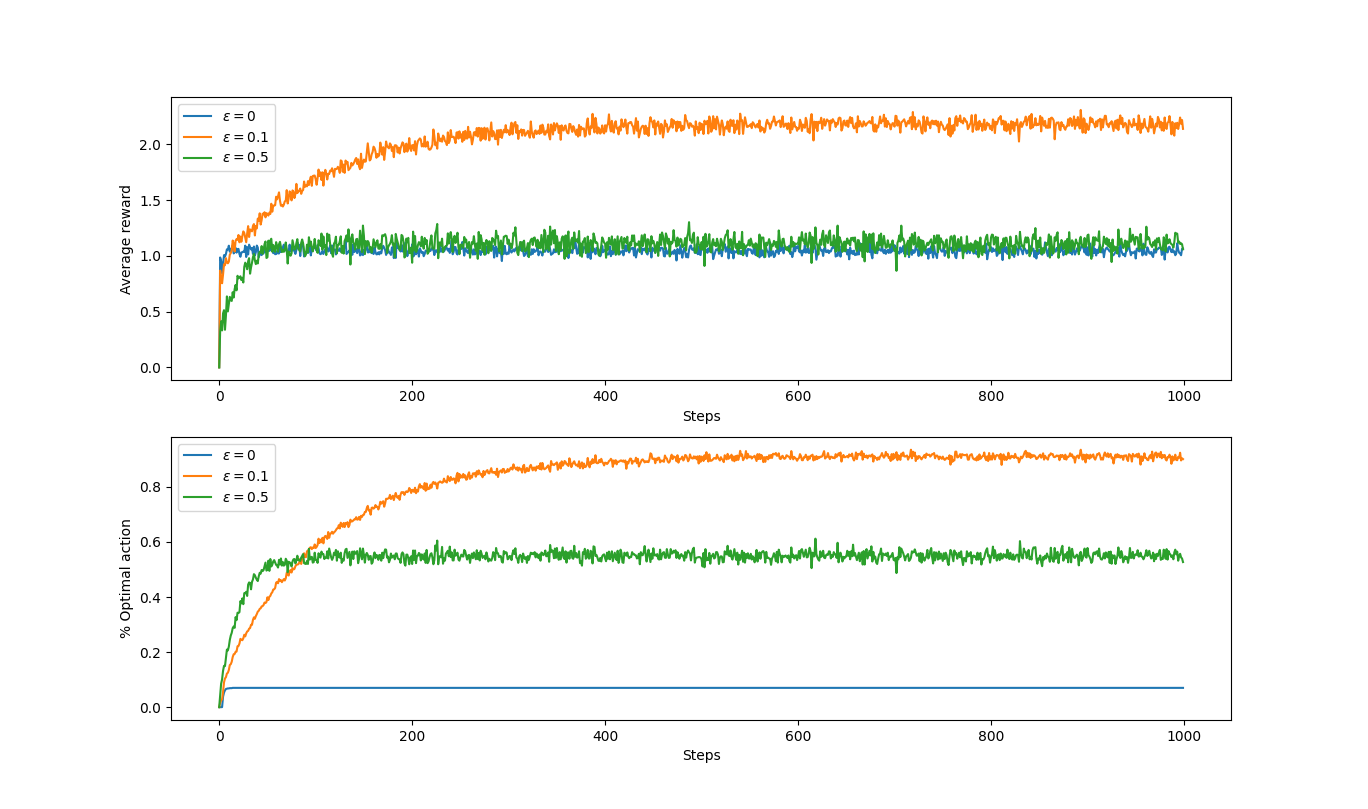
\includegraphics[width = 0.95 \textwidth]{1.4.1.png}    
\end{center}

\end{solution}

% --------------------------------------------------------------------------------

% -------------------------------------------------------------------------------- %

\begin{exercise}

Für welche Werte von $p \in \R$ gibt es ein signiertes Maß $\mu$ auf $(\N, 2^\N)$ mit $\mu(\Bbraces{x}) = x^p (-1)^x$?

\end{exercise}

% -------------------------------------------------------------------------------- %

\begin{solution}

\begin{align*}
    \mu:
        2^N \to \R,
        A \mapsto \sum_{x \in A} x^p (-1)^x
\end{align*}

Die Summe (Reihe) ist für $p < -1$ absolut konvergent, als Minorante der Geometrischen Reihe oder laut dem Leibniz-Kriterium, und $\mu$ damit wohldefiniert, und sonst divergent (nicht gegen $\infty$ oder $-\infty$).

\includegraphicsboxed{MassWHT1&2/MassWHT1&2 - Definition 6.1.png}

\begin{enumerate}

    \item $2^\N$ ist eine Sigmaalgebra.

    \item Der Wertebereich ist entweder $(-\infty, \infty]$ oder $[-\infty, \infty)$, weil
    
    \begin{align*}
        \Forall A \in 2^\N:
            \mu(A) \leq \mu(\N) < \infty.
    \end{align*}

    \item $\mu$ ist sigmaadditiv.
    
    \begin{align*}
        \Forall \vec A := (A_n) \subset 2^\N, ~\text{disjunkt}, A := \bigcup \vec A:
            \mu(A)
            =
            \sum_{x \in A}
                x^p (-1)^x
            =
            \sum_{n \in \N}
                \sum_{x \in A_n}
                    x^p (-1)^x
            \sum_{n \in \N}
                \mu(A_n)
    \end{align*}

\end{enumerate}

\end{solution}

% -------------------------------------------------------------------------------- %

% --------------------------------------------------------------------------------

\begin{exercise}

\phantom{}

\begin{enumerate}[label = (\alph*)]

  \item
  Definieren Sie Ring, Semiring, monotones System, Dynkin-System.
  
  \item
  Gegeben sei der Wahrscheinlichkeitsraum $(\Omega, \mathfrak{S}, \P)$. Für $A \in \mathfrak{S}$ sei
  
  \begin{align*}
    \mathfrak{U}(A) = \Bbraces{B: \P(A \cap B) = \P(A) \P(B)}
  \end{align*}
  
  das System aller Mengen, die von $A$ unabhängig sind. Zeigen Sie, dass $\mathfrak{U}(A)$ ein Dynkin-System ist.

\end{enumerate}

\end{exercise}

% --------------------------------------------------------------------------------

\begin{solution}

(a) Siehe Aufgabe 3 (a) \\

(b)

\begin{itemize}

  \item \Quote{Stabil bzgl. Differenzen von Teilmengen}: Seien $B, C \in \mathfrak{U}(A)$ mit $B \subseteq C$, dann gilt Folgendes.
  \begin{align*}
    \P(A \cap C \setminus B)
    & = \P(A) \P(C \setminus B)
    \Leftrightarrow \\
    \P(A) \P(B) + \P(A \cap C \setminus B)
    & = \P(A) \P(C \setminus B) + \P(A) \P(B)
      = \P(A) \P(C)
    \Leftrightarrow \\
    \P(A \cap C) + \P(A) \P(B)
      =\P(A \cap B) + \P(A) \P(B) + \P(A \cap C \setminus B)
    & = \P(A) \P(C) + \P(A \cap B)
  \end{align*}

  \item \Quote{Stabil bzgl. abzählbaren, disjunkten Vereinigungen}: Sei $(B_n) \in \mathfrak{D}$ disjunkt, dann
  \begin{align*}
    \P \pbraces{A \cap \sum_{n \in \N} B_n}
    =
    \sum_{n \in \N} \P(A \cap B_n)
    =
    \sum_{n \in \N} \P(A) \P(B_n)
    =
    \P(A) \P \pbraces{\sum_{n \in \N} B_n}.
  \end{align*}

  \item \Quote{Enthält Grundmenge}: $\P(A \cap \Omega) = \P(A) = \P(A) \P(\Omega)$

\end{itemize}

\end{solution}

% --------------------------------------------------------------------------------


\printbibliography

\end{document}
